\chapter{مقدمه}
\section{تعریف مسئله}

ترمیم (تکمیل) تصاویر 
\LTRfootnote{Image Inpainting (Completion)}
یکی از شاخه‌های اساسی در حوزه پردازش تصویر است که با هدف بازسازی بخش‌های آسیب‌دیده یا حذف‌شده‌ی تصاویر به گونه‌ای انجام می‌شود که کیفیت بصری و اطلاعات معنایی تصویر حفظ گردد. این مسئله کاربردهای گسترده‌ای در زمینه‌هایی مانند ویرایش تصاویر 
\cite{joSCFEGANFaceEditing2019}
، بازیابی داده‌های تاریخی %
\cite{wanBringingOldPhotos2020, wanOldPhotoRestoration2020}%
، و کاربردهای پزشکی، صنعتی و امنیتی دارد. با این حال، به دلیل پیچیدگی ویژگی‌های بصری تصاویر، مانند الگوهای متقارن، جزئیات دقیق، و بافت‌های پیچیده، ترمیم دقیق و بدون خطا همچنان چالشی بزرگ باقی مانده است.

یکی از مشکلات اصلی در ترمیم تصاویر، حفظ وابستگی‌های طولانی‌مدت در سرتاسر تصویر است. در روش‌های معمولی مانند شبکه عصبی کانولوشنی (CNN)
\cite{laubeImageInpaintingHighResolution2018}%
، که به طور عمده بر ویژگی‌های محلی تمرکز دارند، این وابستگی‌ها به خوبی مدیریت نمی‌شوند. به این معنا که در مواقعی که نواحی بزرگی از تصویر نیاز به ترمیم دارند یا لبه‌های پیچیده‌ای باید بازسازی شوند، مدل‌های CNN قادر به درک کامل و منطقی از بافت کلی تصویر نبوده و ممکن است در تولید نواحی ترمیم‌شده دچار مشکلاتی مانند عدم هماهنگی با محیط اطراف شوند. این مشکل به‌ویژه در ترمیم نواحی بزرگ یا پیچیده‌تر از تصویر که نیاز به درک زمینه و روابط بین نواحی مختلف دارند، خود را نشان می‌دهد. به همین دلیل، استفاده از معماری‌های ترنسفورمر (Transformer)
\cite{vaswaniAttentionAllYou2023}
که از مکانیزم توجه
\LTRfootnote{Attention Mechanism}
\cite{bahdanauNeuralMachineTranslation2016}
 برای شناسایی وابستگی‌ها در سطح سراسری بهره می‌برد، می‌تواند این مشکل را به طور مؤثری حل کند. ترنسفورمر ها  که به دلیل مکانیزم توجه خود عملکرد موفقی در زمینه‌های مختلف یادگیری عمیق داشته اند، می توانند با توانایی پردازش وابستگی‌های بلندمدت، قادرند اطلاعات مورد نیاز از سرتاسر تصویر را جمع‌آوری کرده و نواحی ترمیم‌شده را به شکلی هم‌راستا و منطقی با بقیه تصویر بازسازی کنند. یک مثال از رابطه ای تصویری که «بلند مدت‌» طلقی می‌شود در شکل \ref{fig:longterm} قابل مشاهده است.
 
 \begin{figure}
 	\centering
 	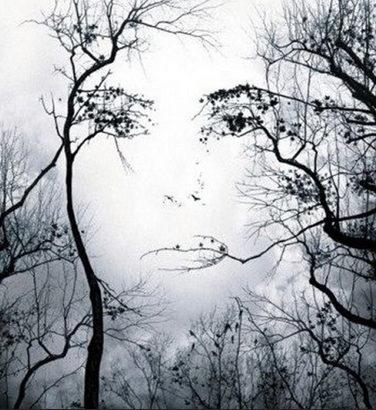
\includegraphics[width=0.7\linewidth]{longterm}
 	\caption{یک نمونه تصویر با «وابستگی بلندمدت» منظور آن است که دیدگاه محلی به بخش های مختلف معنای خاصی منتقل نمی‌کند اما هنگام مشاهده تصویر و در نظر گرفتن کامل روابط دورادور شاخه ها، یک الگوی چهره نمایان می‌شود.}
 	\label{fig:longterm}
 \end{figure}
 

\section{اهمیت موضوع}
اهمیت مسئله ترمیم تصاویر از آنجا ناشی می‌شود که این فرایند به‌طور مستقیم با کیفیت تجزیه و تحلیل و تفسیر داده‌های بصری در بسیاری از زمینه‌ها مرتبط است. در کاربردهای پزشکی، مانند بازسازی تصاویر پزشکی از سی‌تی‌اسکن‌ها یا MRI‌ ها، ترمیم تصاویر می‌تواند به تشخیص دقیق‌تر و سریع‌تر بیماری‌ها کمک کند. همچنین، در زمینه‌های امنیتی و نظارتی، بازسازی صحیح و دقیق تصاویر از محیط‌های آسیب‌دیده می‌تواند اطلاعات حیاتی برای تجزیه و تحلیل وقایع فراهم آورد. در دنیای دیجیتال امروزی، ترمیم تصاویر به‌عنوان یکی از ابزارهای اساسی در ویرایش گرافیکی و بازسازی آثار هنری تاریخی شناخته می‌شود.


\section{اهداف پژوهش}

در این تحقیق، هدف اصلی بررسی کاربرد معماری‌های ترنسفورمر در حوزه ترمیم تصاویر است. یکی از چالش‌های بزرگ در ترمیم تصاویر، توانایی مدل‌ها در حفظ همبستگی‌های بلندمدت و منطقی در سراسر تصویر است. در حالی که شبکه‌های CNN معمولاً برای استخراج ویژگی‌های محلی مناسب هستند، مشکل آنها در مدیریت وابستگی‌های بلندبرد و ایجاد همبستگی‌های طبیعی در نواحی بزرگ تصویر مشهود است.

یکی دیگر از اهداف تحقیقاتی، بررسی چگونگی استفاده از مدل‌های ترنسفورمر برای بهبود کارایی و سرعت فرآیند ترمیم است. در حالی که مدل‌های RNN و LSTM در گذشته برای پردازش داده‌های ترتیبی استفاده می‌شدند، این مدل‌ها در پردازش داده‌های غیر ترتیبی مانند تصاویر با مشکل مواجه هستند. به طور خاص، این مدل‌ها به دلیل پردازش ترتیبی و وابستگی به مراحل قبلی، زمان‌بر و کند هستند. در مقابل، ترنسفورمر ها با پردازش موازی داده‌ها، به مدل‌ها این امکان را می‌دهد که به طور کارآمدتری پردازش کنند و زمان پردازش را برای تصاویر با ابعاد بزرگ کاهش دهند. این تحقیق به دنبال ارزیابی این مزیت برای ترمیم تصاویر است.

یکی از اهداف فرعی تحقیق، تحلیل و مقایسه عملکرد ترنسفورمر با سایر روش‌های رایج در ترمیم تصاویر مانند GAN و U-Net است. در حالی که مدل‌های GAN در تولید تصاویر از کیفیت بالایی برخوردارند، از نظر پایداری در فرآیند آموزش و توانایی برای ترمیم نواحی بزرگ و پیچیده، همچنان با مشکلاتی مواجه هستند. همچنین، U-Net که یکی از مدل‌های موفق در ترمیم تصویر است، بیشتر به ویژگی‌های محلی توجه دارد و گاهی در ترمیم نواحی بزرگ‌تر یا پیچیده‌تر دچار مشکلاتی می‌شود. تحقیق حاضر به دنبال نشان دادن مزایای ترنسفورمر در رفع این مشکلات و ارائه یک راهکار پیشنهادی با نتایج بهبود یافته است.

%در نهایت، این تحقیق با ارائه رویکردهایی برای ترکیب معماری‌های مختلف، مانند LSTM و ترنسفورمر در ترمیم تصاویر، به دنبال شناسایی الگوهای جدیدی برای بهبود عملکرد مدل‌ها است. یکی از جنبه‌های مهم این تحقیق، ارزیابی نتایج با استفاده از معیارهای معتبر همچون SSIM و PSNR است تا اثبات کند که تغییرات معماری پیشنهادی در نهایت به بهبود کیفیت ترمیم تصاویر می‌انجامد. همچنین، آزمایش‌های ناموفق قبلی با LSTM در ترمیم غیرزمانی به طور مفصل بررسی خواهد شد تا بینش‌های جدیدی از آن‌ها استخراج گردد و به توسعه مدل‌های آینده کمک کند.


\section{ساختار پایان‌نامه}

این پایان‌نامه در پنج فصل تنظیم شده است که هرکدام به جنبه‌های مختلف تحقیق و تحلیل مدل‌های ترمیم تصویر می‌پردازد. در ادامه، در فصل دوم، مسئله ترمیم تصویر را فرموله و مدل‌سازی می‌کنیم و مفاهیم کلیدی مرتبط با ترمیم تصویر و  روش های یادگیری را بیان می‌کنیم. معیار های ارزیابی، شبکه های عمیق، شبکه های کاملا متصل، توابع فعال سازی و توابع هزینه شرح داده می‌شوند و در فصل های آینده استفاده خواهند شد. در فصل سوم، مروری بر مطالعات، روش‌ها و مجموعه داده‌های%
\LTRfootnote{Datasets}
ترمیم تصویر و تاریخچه روش‌های ترمیم تصویر انجام می‌شود. روش های الگوریتمی بررسی شده و نیاز به روش های یادگیری توجیه می‌شود. سپس چند روش مبتنی بر یادگیری بررسی می‌شوند. در این فصل همچنین به تحلیل مزایا و معایب این روش‌ها پرداخته خواهد شد و لزوم استفاده از روش هایی  با حفظ وابستگی بلند مدت توجیه می‌شود. فصل چهارم، تاریخچه ترجمه ماشینی و شبکه های بازگشتی را توضحی داده، سپس مکانیزم توجه را معرفی کرده و توضیح می‌دهد و به صورت جامع ترنسفورمر ها را شرح می‌دهد. در نهایت فصل پنجم یک روش پیشنهادی الهام گرفته از ViT را ارائه داده و بررسی می‌کند.
%در نهایت، در فصل پنجم نتایج را بررسی و جمع‌بندی می‌کنیم و پیشنهاداتی برای بهبود روش‌های آتی ارائه می‌دهیم.